\documentclass{standalone}
\usepackage{tikz}
\begin{document}
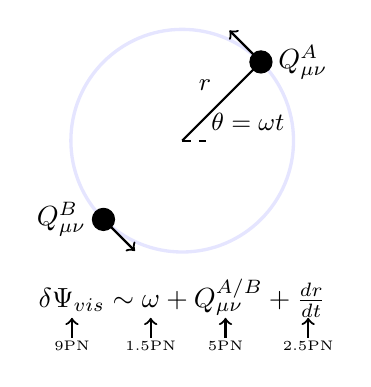
\begin{tikzpicture}
    %\node[] at (0,1.7) {\small{$\delta h_{+,\times}(t)\approx A_{GR}(t) \exp\left(i\delta\Psi_{vis} t\right)$}};
    \filldraw[color=blue!10, fill=white, very thick](0,0) circle (1.414);
    \draw[thick    ] ( 0, 0) -- node[above left] {\small{$r$}} ++ (1,1);
    \draw[thick,dashed] ( 0, 0) -- node[above right] {\small{$\;\theta=\omega t$}} ++ (0.3,0);
    \filldraw[black] ( 1, 1) circle (4pt) node[right] { $\;Q^A_{\mu\nu}$};
    \draw[thick, ->] ( 1, 1) -- ( 0.6, 1.4);
    \filldraw[black] (-1,-1) circle (4pt) node[left] { $Q^B_{\mu\nu}\;$};
    \draw[thick, ->] (-1,-1) -- (-0.6,-1.4) ;
    \node[] at (0,-2) {$\delta \Psi_{vis} \sim\omega+Q^{A/B}_{\mu\nu}+\frac{dr}{dt}$};
    \draw[thick, ->] (-1.4,-2.5) -- (-1.4,-2.25);
    \node[] at (-1.4,-2.6) {\tiny{9PN}};
    \draw[thick, ->] (-0.4,-2.5) -- (-0.4,-2.25);
    \node[] at (-0.4,-2.6) {\tiny{1.5PN}};
    \draw[thick, ->] (0.55,-2.5) -- (0.55,-2.25);
    \node[] at (0.55,-2.6) {\tiny{5PN}};
    \draw[thick, ->] (1.6,-2.5) -- (1.6,-2.25);
    \node[] at (1.6,-2.6) {\tiny{2.5PN}};
    \end{tikzpicture}
\end{document}
